\documentclass[a4paper,11pt]{article}

\usepackage[utf8]{inputenc}
\usepackage[italian]{babel}
\usepackage{indentfirst}
\usepackage[margin=2.2cm]{geometry}
\usepackage[most]{tcolorbox}
\usepackage{graphicx}
\usepackage{hyperref}
\usepackage[italian]{varioref}
\usepackage{listings}
\usepackage{xcolor}
\usepackage[numbered,framed]{matlab-prettifier}

\graphicspath{{figures/}}


\title{\textbf{Perceptron Monostrato}}
\author{Lara Vignotto}
\date{\today}


\begin{document}

\maketitle
\vspace{.5cm}


%%%%%%%%%%%%%%%%%%%%%%%%%%%%%%
\section{Introduzione e Implementazione}

Viene qui presentata l'implementazione di un \emph{perceptron monostrato}. Si tratta di una rete neurale molto semplice che si comporta come una porta logica \texttt{OR}. È composta da un \emph{input layer} con due nodi collegati all'unico nodo dell'\emph{output layer}.

Il pacchetto per il perceptron è composto da 2 script e 2 funzioni:

\begin{itemize}
    \item \textbf{Script}:
    \begin{itemize}
        \item \texttt{Perc\_Training}: viene definita la procedura di apprendimento per il perceptron. Utilizza la \texttt{SGD\_DeltaRule\_Function}, e genera un file con una matrice dei valori dei pesi calcolati a seguito dell'apprendimento;
        \item \texttt{OR\_Test\_network}: una volta ottenuti i pesi, applica la procedura di apprendimento del perceptron monostrato. Restituisce in output i valori attesi in corrispondenza di ciascun input, in questo caso un vettore di quattro 0 e 1 a seconda della combinazione di bit a due a due data in input.
    \end{itemize}

    \item \textbf{Funzioni}:
    \begin{itemize}
        \item \texttt{SGD\_DeltaRule\_Function}: applica la Generalized Delta Rule (GDR). Viene utilizzata ripetutamente nella fase di apprendimento (in \texttt{Perc\_Training}) per modificare i valori dei pesi. Questa ripetuta modifica serve a diminuire l'errore, ovvero la differenza tra il valore osservato e quello atteso;
        \item \texttt{Sigmoid}: applica la funzione sigmoide come funzione di attivazione. Viene utilizzata in \texttt{OR\_Test\_network}.
    \end{itemize}
\end{itemize}

\noindent Analizziamo in dettaglio le quattro procedure.


%%%%%%%%%%%%%%%
\subsection{Perc\_Training}

\begin{lstlisting}[style=Matlab-editor,title=\texttt{Perc\_Training.mat}]
% Vettori di input (training set)
input = [0 0;
         0 1;
         1 0;
         1 1;
            ];

% Valori attesi in output
correct_output = [0
                  1
                  1
                  1
                   ];

% Bias
OR_bias = -3;
% Inizializzazione casuale dei pesi
OR_Weight = 2 * rand(1, 2) - 1;
% Iperparametro con numero di epoche
N_epoch = 1000;

% Ciclo di apprendimento
for epoch = 1:N_epoch
    OR_Weight = SGD_DeltaRule_Function(OR_Weight, OR_bias, input, correct_output);
end

% Memorizzazione su file dei pesi calcolati
save('OR_Trained_Network.mat');
\end{lstlisting}

Inizialmente vengono dichiarati come matrice i quattro vettori di input, ognuno corrispondente ad una riga di due elementi (l.~\texttt{2-6}). In questo caso sono le quattro combinazioni di 2 bit, in quanto si vuole che il perceptron si comporti come una porta logica \texttt{OR}. Successivamente vengono assegnati i valori attesi in output in corrispondenza di ciascun input (l.~\texttt{9-13}). Seguono il valore del bias $b$, l'inizializzazione casuale dei pesi, e l'iperparametro col numero di epoche (l.~\texttt{16-20}).

Si esegue il ciclo di apprendimento della rete (l.~\texttt{23-25}): per un numero di volte corrispondente al numero di epoche si applica al vettore peso la regola di apprendimento Generalized Delta Rule (GDR) (cfr. \nameref{sgd-drf}).

Infine, i pesi così calcolati vengono salvati nel file \texttt{OR\_Trained\_Network.mat}.


%%%%%%%%%%%%%%%
\subsection{SGD\_DeltaRule\_Function}\label{sgd-drf}

\begin{lstlisting}[style=Matlab-editor,title=\texttt{SGD\_DeltaRule\_Function.mat}]
function OR_Weight = SGD_DeltaRule_Function(OR_Weight, OR_bias, input, correct_output)
%   Iperparametro per regolare la velocita' di apprendimento
    alpha = 0.8;
%   Numero dei vettori di input (4)
    N = size(input, 1);

    for k = 1:N 
        transposed_input = input(k, :)';
        corval = correct_output(k);
        weighted_sum = OR_Weight * transposed_input + OR_bias;
        output = Sigmoid(weighted_sum);
        error = corval - output;
        delta = output * (1 - output) * error;
        dWeight = alpha * delta * transposed_input;
        OR_Weight = OR_Weight + dWeight';
    end	
end
\end{lstlisting}
Questa funzione implementa un metodo di discesa lungo il gradiente chiamato \textbf{Generalized Delta Rule (GDR)}.


%%%%%%%%%%%%%%%
\subsection{Sigmoid}\label{sig}

\begin{lstlisting}[style=Matlab-editor,title=\texttt{Sigmoid.mat}]
function y = Sigmoid(x)
    y = 1/(1+exp(-x));
end
\end{lstlisting}


%%%%%%%%%%%%%%%
\subsection{OR\_Test\_network}

\begin{lstlisting}[style=Matlab-editor,title=\texttt{OR\_Test\_network.mat}]
load('OR_Trained_Network.mat')

N = 4;
for k = 1:N
    transposed_input = input(k, :)';
    weighted_sum = OR_Weight * transposed_input + OR_bias;
    output = Sigmoid(weighted_sum)
end
\end{lstlisting}

Caricato il file con i valori dei pesi calcolati nel primo script, applica la procedura di apprendimento. Per ogni vettore di input viene restituito un output definito dalla \textbf{funzione di attivazione sigmoide} (cfr. \nameref{sig}). In particolare, la funzione sigmoide mappa il valore che deve essere restituito in output in un valore compreso tra 0 e 1.



%%%%%%%%%%%%%%%%%%%%%%%%%%%%%%
\section{Risultati}

Lanciando prima \texttt{Perc\_Training.mat} e di seguito \texttt{OR\_Test\_network.mat} vengono stampati a schermo i quattro valori di output:

\begin{lstlisting}[style=Matlab-editor]
output =

    0.0474


output =

    0.9735


output =

    0.9734


output =

    1.0000
\end{lstlisting}

Essendo l'output atteso \texttt{0,1,1,1} si può affermare che i valori in output ottenuti sono corretti: il perceptron si comporta come una porta logica \texttt{OR}.


%%%%%%%%%%%%%%%%%%%%%%%%%%%%%%
\section{Errori e Monitoraggio dell'Apprendimento}

%%%%%%%%%%%%%%%
\subsection{Mean Squared Error e Learning Curve (Loss)}

Per valutare l'errore, utilizziamo il \textbf{Mean Squared Error (MSE)} (errore quadratico medio). Si tratta della differenza media al quadrato fra output effettivo e output corretto. In Matlab il MSE si può calcolare con la funzione \texttt{immse}. Per effettuare il \textbf{monitoraggio dell'apprendimento} si può calcolare il MSE ad ogni epoca e tracciarne il grafico. La curva risultante è detta \textbf{learning curve} (curva di apprendimento) o \textbf{loss curve}.

Si modifica quindi \texttt{SGD\_DeltaRule\_Function} in modo tale che restituisca anche il vettore di output calcolati, in modo che in \texttt{Perc\_Training} si possano calcolare i dati necessari a costruire il grafico della curva di apprendimento:

\begin{lstlisting}[style=Matlab-editor,title=\texttt{SGD\_DeltaRule\_Function.mat}]
function [OR_Weight,output0] = SGD_DeltaRule_Function(OR_Weight, OR_bias, input, correct_output)
    ...
    output0 = [];

	for k = 1:N 
        ...
        output = Sigmoid(weighted_sum);
        output0 = [output0 output];
        ...
	end	
end	
\end{lstlisting}

\begin{lstlisting}[style=Matlab-editor,title=\texttt{Perc\_Training.mat}]
...
MSE0 = [];      % MSE per epoch
epoch0 = [];    % epoch_a
for epoch = 1:N_epoch
        [OR_Weight,output0] = SGD_DeltaRule_Function(OR_Weight, OR_bias, input, correct_output);

%   Dati per il grafico della curva di apprendimento (loss)
    MSE = immse(correct_output, output0');  % Mean Squared Error
    MSE0 = [MSE0 MSE];
    epoch0 = [epoch0 epoch];
end

% Figura con il grafico della curva di apprendimento (loss)
figure();
plot(epoch0(1:300),MSE0(1:300)), grid;
title('Learning Curve (Loss)')
xlabel('epoch')
ylabel('MSE')
...
\end{lstlisting}

\begin{figure}[htb]
    \centering
    \tcbox[boxrule=.3mm,colback=white]{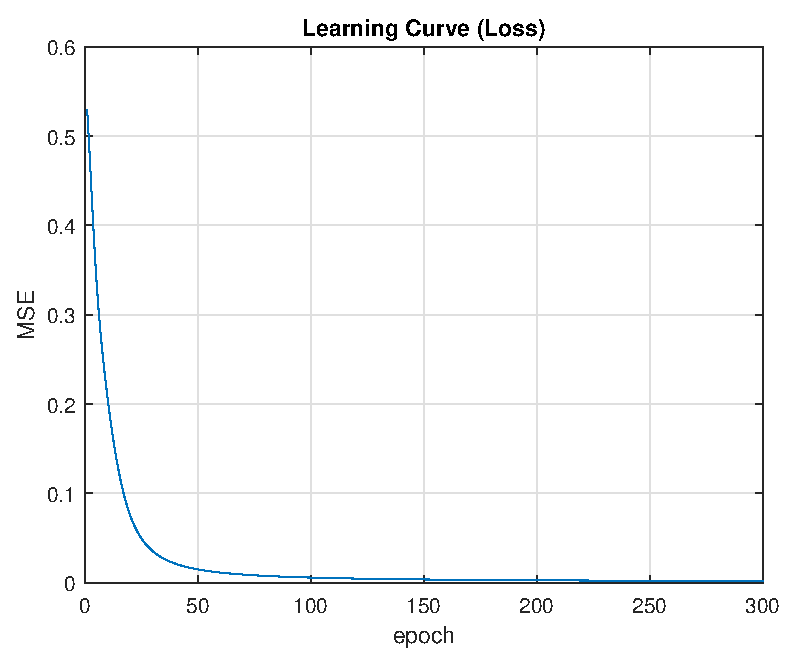
\includegraphics[width=.9\textwidth]{epsFig1}}
    \caption{Curva di apprendimento.}
    \label{fig1}
\end{figure}

In Figura \vref{fig1} si può osservare il grafico della curva di apprendimento. Si nota come il MSE diminuisca (rapidamente) all'aumentare del numero di epoche. Il repentino calo dell'errore significa che l'\textbf{apprendimento è veloce}.


%%%%%%%%%%%%%%%
\subsection{Weight}

Si vuole analizzare la curva di apprendimento dei pesi. Ad ogni epoca vengono calcolati i pesi, quindi in \texttt{Perc\_Training} si possono raccogliere in due vettori i valori dei pesi e tracciare il loro andamento in funzione delle epoche:

\begin{lstlisting}[style=Matlab-editor,title=\texttt{Perc\_Training.mat}]
...
Weight1 = [];   % Weight per epoch (1)
Weight2 = [];   % Weight per epoch (2)
for epoch = 1:N_epoch
        [OR_Weight,output0] = SGD_DeltaRule_Function(OR_Weight, OR_bias, input, correct_output);

%   Dati per il grafico dei pesi
    Weight1 = [Weight1 OR_Weight(1)];
    Weight2 = [Weight2 OR_Weight(2)];
    epoch0 = [epoch0 epoch];
end

% Figura delle curve di apprendimento W1, W2
% grafico peso 1
figure('Name', 'Curva Loss dei Pesi');
subplot(1,2,1);
plot(epoch0(1:500),Weight1(1:500)), grid;
title('Grafico dei Pesi 1')
xlabel('epoch')
ylabel('Weight1')
% grafico peso 2
subplot(1,2,2)
plot(epoch0(1:500),Weight2(1:500)), grid;
title('Grafico dei Pesi 2')
xlabel('epoch')
ylabel('Weight2')
...
\end{lstlisting}

La Figura \vref{fig2} mostra come il valore dei pesi aumenta all'avanzare delle epoche, fino ad ``appiattirsi'' ad un valore di poco superiore a 6. La convergenza delle curve ad un valore significa che nel tempo sono stati appresi i fattori peso delle connessioni. Questo andamento era prevedibile: l'apprendimento migliora con il passare delle epoche.

\begin{figure}[htb]
    \centering
    \tcbox[boxrule=.3mm,colback=white]{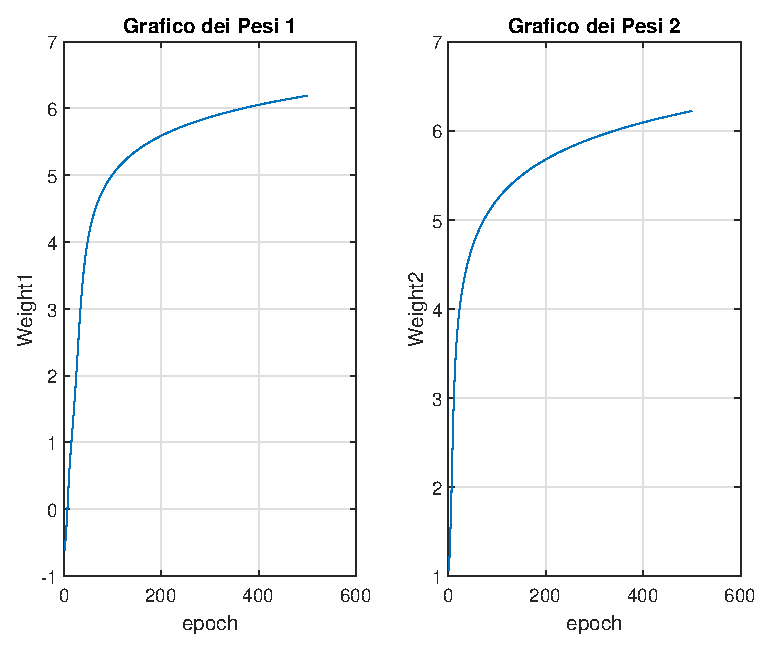
\includegraphics[width=.9\textwidth]{epsFig2}}
    \caption{Curva di apprendimento dei pesi.}
    \label{fig2}
\end{figure}


%%%%%%%%%%%%%%%
\subsection{Learning Rate}

La dipendenza dal parametro $\alpha$ è detta \textbf{learning rate} (tasso di apprendimento). Per studiarne l'andamento si possono produrre cinque curve loss, ognuna per un diverso valore di $\alpha$.

Si modifica \texttt{SGD\_DeltaRule\_Function} in modo che accetti un ulteriore parametro, \texttt{alpha}. In \texttt{Perc\_Training} si dichiarano i cinque valori di $\alpha$ che si vogliono analizzare --in questo caso $0.1$, $0.3$, $0.5$, $0.7$, $0.9$-- e si introduce un ciclo \texttt{for} esterno che cicla sui cinque $\alpha$. Ad ogni ciclo si produce la curva loss relativa all'apprendimento della rete neurale e la si aggiunge ad un grafico. La figura risultante conterrà cinque curve, ognuna corrispondente ad un valore di $\alpha$.

\begin{lstlisting}[style=Matlab-editor,title=\texttt{SGD\_DeltaRule\_Function.mat}]
function [OR_Weight,output0] = SGD_DeltaRule_Function(alpha, OR_Weight, OR_bias, input, correct_output)
    ...
end	
\end{lstlisting}

\begin{lstlisting}[style=Matlab-editor,title=\texttt{Perc\_Training.mat}]
alpha = [0.1 0.3 0.5 0.7 0.9];
for i = alpha
    input = ... 
    ...
    MSE0 = [];      % MSE per epoch
    epoch0 = [];    % epoch_a
    for epoch = 1:N_epoch
            [OR_Weight,output0] = SGD_DeltaRule_Function(i, OR_Weight, OR_bias, input, correct_output);

        MSE = immse(correct_output, output0');  % Mean Squared Error
        MSE0 = [MSE0 MSE];
        epoch0 = [epoch0 epoch];
    end

    plot(epoch0(1:300),MSE0(1:300)), grid;
    title('Learning Curve (Loss)')
    xlabel('epoch')
    ylabel('MSE')
    legend('alpha 0.1', 'alpha 0.3', 'alpha 0.5', 'alpha 0.7', 'alpha 0.9');
    hold on
end
...
\end{lstlisting}

In Figura \vref{fig3} si può osservare il grafico delle curve di apprendimento al variare di $\alpha$. Si nota come più $\alpha$ è basso e più l'apprendimento è lento, e viceversa. Ci si aspettava un comportamento di questo tipo: il parametro $\alpha$ rappresenta il tasso di apprendimento, e regola la velocità alla quale una rete neurale effettua l'apprendimento.

\begin{figure}
    \centering
    \tcbox[boxrule=.3mm,colback=white]{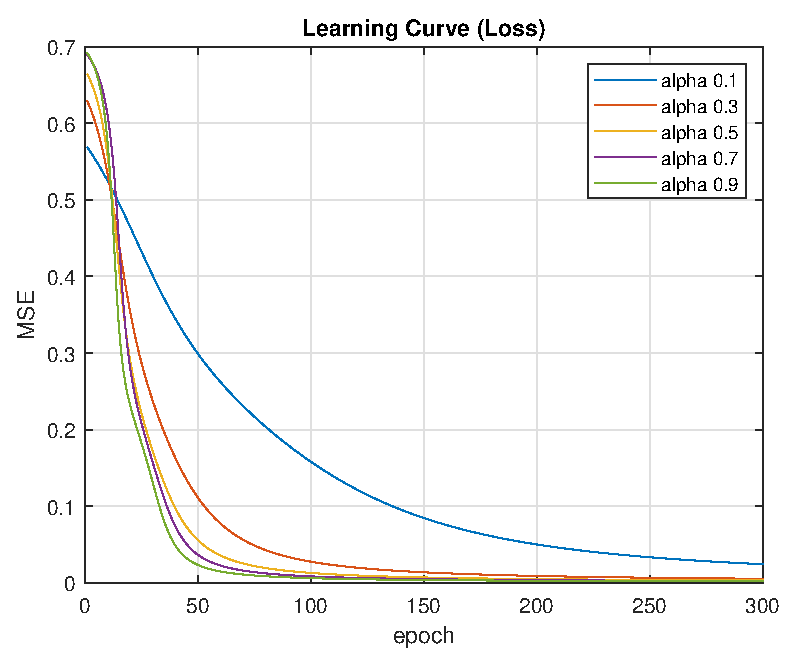
\includegraphics[width=.9\textwidth]{epsFig3}}
    \caption{Curve di apprendimento al variare di $\alpha$.}
    \label{fig3}
\end{figure} 


\end{document}